\section{Metachem grid}

The Metachem grid is a project for producing ``a meta-laboratory for code
integration in \textit{ab initio} methods''. The project, still in
development, has been carried on under the D23 COST action \cite{cost-site},
with the objective to develop a common grid infrastructure where
computational chemists can access several \textit{ab initio} codes produced
by different laboratories through a simple and user-friendly interface.

Most of the interested parties developed quantum chemistry codes for
{Post-SCF} evaluations, mainly for internal research. These techniques can be
integrated in a common infrastructure, but with the requisite to leave each code
on the platform it was originally designed for, under the responsibility of
its owner for maintenance and production. This will distribute the
administrative burden and avoid binary code duplication.

Finally, a set of standard quantum chemistry codes (\texttt{MOLCAS},
\texttt{COLUMBUS} or \texttt{DALTON}) must be integrated into the grid to
provide commonly used entities, like integrals, overlap, CASSCF orbitals and
wavefunctions, and so on.

Various considerations, ranging from technical factors to license
restrictions prevent direct changes to existing codes. A more conservative
strategy has been considered, at least in the initial deployment of the
project (see Fig.~\ref{fig:wrapper-scheme}): input and output wrappers
convert files and workflow logic between the local environment of a given
program and the shared grid environment, and viceversa. Input wrappers
convert information provided by the grid to low-level input such as Fortran
namelists and proprietary binary files. Output wrappers parse the products
of the program and create the standard information which will return to the
grid.

\begin{center}
\begin{figure}[ht]
\begin{center}
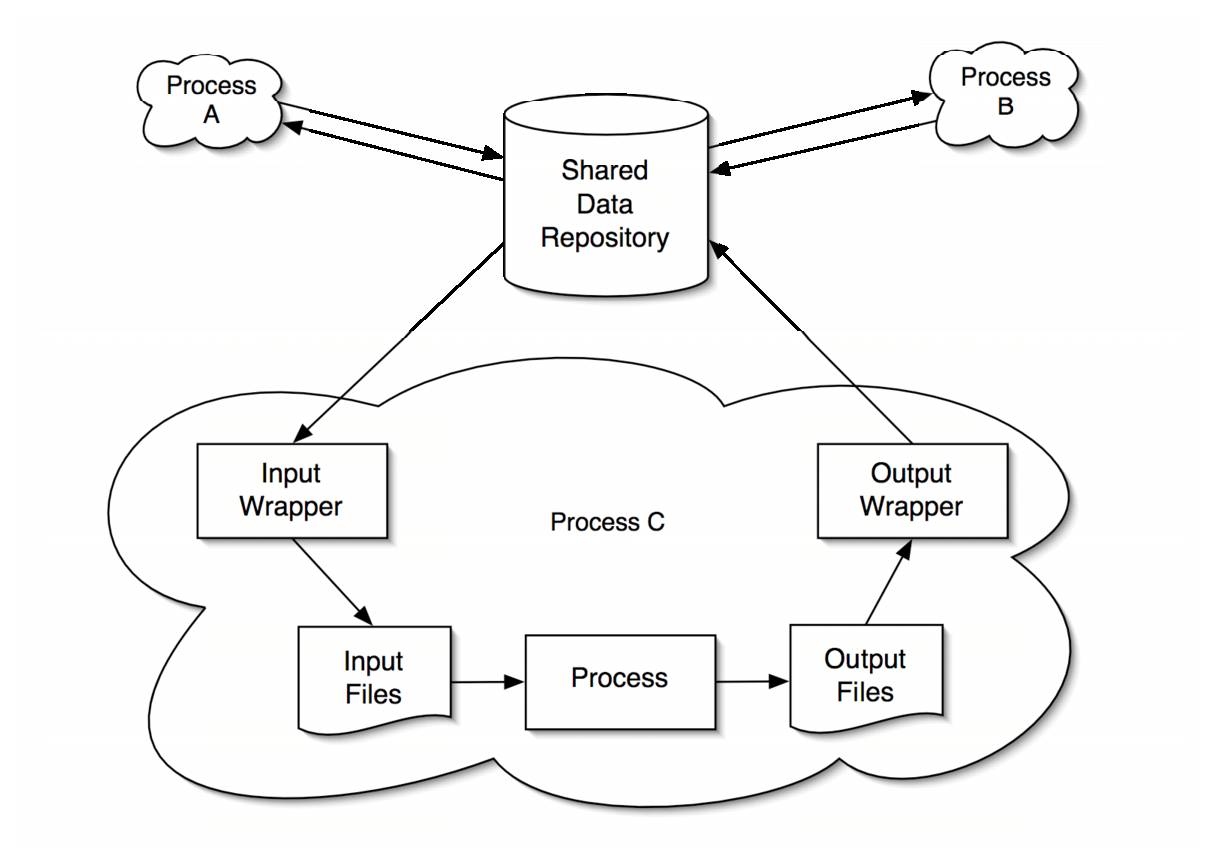
\includegraphics[width=10cm,keepaspectratio]{04_grid/images/wrapper-scheme-gimped.eps}
\end{center}
\caption{\footnotesize A scheme for the data handling inside a single
calculation environment. Data are made available by the data repository,
adapted to the local input environment of the process. The result is
converted back to the standard format and returned to the repository.}
\label{fig:wrapper-scheme}
\end{figure}
\end{center}


This strategy imposes the development and maintenance of the wrappers by
the interested parties. They are supposed to track the changes of their own
codes and adapt the wrappers accordingly. For historical reasons,
the reference language for the development of these wrappers is Fortran. 

The shared environment must also agree on a common file format.  Due to the
nature of the project, this common file format must be platform independent,
code independent, and easy to debug. Two different kinds of information have
been identified in quantum chemistry calculations:
\begin{itemize}
\item \textit{small data}, mainly ASCII encoded, like atom labels, geometry,
symmetry, basis sets, but also workflow specific information
\item \textit{large data}, normally binary encoded, like integrals and expansion coefficients
\end{itemize}

For the first kind of data, many initiatives are active nowadays. The more
extensive is the work of Murray-Rust et al.\cite{jcics-39-928-1999,
jcics-41-1113-2001,jcics-41-1124-2001,cc-1471-2000,njc-618-2001} with the
development of CML (Chemistry Markup Language) under the eScience project in
UK. The choice of XML allows both human readability and machine parsing.

Unfortunately, CML does not provide direct support for quantum chemical
entities.  After a brief analysis of the problem, an experimental
\textit{XML-schema} for quantum chemistry entities, QCML (Quantum Chemistry
Markup Language) has been deployed. The parsing of this information in
Fortran is possible through a library, named F77/F90xml, specifically
developed for the project.

For the second kind of data (large binary data) XML is not a good
technology, mainly due to its verbosity. For several reasons,
HDF5\cite{hdf5-site} is considered the best technology for large binary
data.

The next step, to be done in the future, is the definition and setup of
user defined workflows based on heterogeneous codes, located on different
platforms, communicating through the common formats. The actual technology
has yet to be chosen, but the choice seems to be oriented towards
UNICORE\cite{streit-tbp-2005,erwin-unicore,unicore-site}, together with a
common language for describing both workflow and intrinsic differences
between work paths. 

The final infrastructure is expected to satisfy both grid requirements
(fault tolerance, reliability) and human interface requirements (access via
web interface or specialized clients). An access point to grid services will be provided by
the CINECA supercomputing center. Its role is to coordinate the federated
system, where each node provides one or more services to the grid.

